\documentclass[a4paper, 11pt]{article}
\usepackage{amsmath, amssymb, amsthm}
\usepackage{xeCJK}
\usepackage{fontspec}
\usepackage{xunicode}
\usepackage{xltxtra}
\usepackage{graphicx}

\setCJKfamilyfont{tt}{SimSun}
\setmainfont{SimSun} 		%默认字体,默认英文字体。
\setCJKmainfont{SimSun} 		%中文默认字体
\setCJKmonofont{SimSun}
\CJKsetecglue{} 			%中英间隔

%\XeTeXlinebreaklocale "zh"  % 表示用中文的断行
%\XeTeXlinebreakskip = 0pt plus 1pt % 多一点调整的空间设置字体。

\newcommand{\cn}{\fontspec{Courier New}}
%字体大小
\newcommand{\ltwo}{\fontsize{18pt}{27pt}\selectfont} 		%小二
\newcommand{\three}{\fontsize{16pt}{24pt}\selectfont}		%三号
\newcommand{\lthree}{\fontsize{15pt}{22.5pt}\selectfont}	%小三
\newcommand{\four}{\fontsize{14pt}{21pt}\selectfont}		%四号
\newcommand{\lfour}{\fontsize{13pt}{18pt}\selectfont}		%小四
\newcommand{\five}{\fontsize{10.5pt}{15.75pt}\selectfont}	%五号
\newcommand{\lfive}{\fontsize{9pt}{13.5pt}\selectfont}		%小五

\usepackage{listings}
\lstset{language=Java}%这条命令可以让LaTeX排版时将C++键字突出显示
\lstset{breaklines}%这条命令可以让LaTeX自动将长的代码行换行排版
%\lstset{extendedchars=false}%这一条命令可以解决代码跨页时,章节标题,页眉等汉字不显示的问题
\lstset{xleftmargin=28pt}
\lstset{tabsize=4}
\lstset{escapechar=`} %中文注释问题
\lstset{columns=flexible}
\lstset{basicstyle=\cn\lfive}

%图,表标题的间距。
\usepackage{caption}
\setlength{\abovecaptionskip}{10pt}
\setlength{\belowcaptionskip}{0pt}
\usepackage{tabularx}

\renewcommand {\tablename}{\five 表}
\renewcommand {\thetable}{\arabic{table}}
\usepackage{booktabs}
\renewcommand {\heavyrulewidth}{1.5pt}	%表格外线宽
\renewcommand {\lightrulewidth}{1pt}	%表格内线宽

\captionsetup{labelsep=space}

\theoremstyle{plain}\newtheorem{Lemma}{定理}
%%%%%%%%%%%%%%%%%%%%%%%%
%%%%%%%%%%%正文%%%%%%%%%%
%%%%%%%%%%%%%%%%%%%%%%%%
\begin{document}

\title{{\Huge 算法分析与设计第五次作业\\}}
\author{黄丛宇 2010212439}
\date{\today}

\maketitle

\section{实验环境}
\begin{itemize}
	\item CPU: Intel(R) Core(TM)2 Duo CPU T5870 2.00GHz
	\item MEM: 1GB
	\item OS : Debian 5.0 (1GB swap)
	\item Java: java version "1.6.0\_21"
\end{itemize}
\section{Exercise 15.5-4}
由于$root[i,j-1]\le root[i,j]\le root[i+1,j]$,因此,算法的最内层循环不需要从i循环到j,
而只需从root[i,j-1]循环到root[i+1,j]。算法如下:
\begin{verbatim}
Optimal-Adv-BST(p,q,n)
    for i <- 1 to n+1
    do
        e[i, i-1] <- qi-1
        w[i, i-1] <- qi-1
    for i <- 1 to n
        do 
            root[i,i] <- i
    for k <- 1 to n
        do
            for i <- 1 to n-k+1
                do
                    j <- i+k-1
                    e[i,j] <- ∞
                    w[i,j] <- w[i,j-1]+pj+qj
                    for r <- root[i,j-1] to root[i+1, j]
                            do
                                t <- e[i, r-1]+e[r+1,j]+w[i,j]
                                if t < e[i,j]
                                    then 
                                        e[i,j] <- t
                                        root[i,j] <- r
    return e and root
\end{verbatim}

对于上面的算法,时间复杂度为:
\begin{align*}
	n\sum_{k \le j \le n, i=j-k}^{}(root[i+1,j]-root[i,j-1]+1)\\
	=n(root[n-k+1,n]-root[0,k-1]+n-d+1)
	\le 2n^2
	=O(n^2)
\end{align*}  	
所以,改进后的算法复杂度为$O(n^2)$。


\section{Exercise 16.2-2 knapsack}
对于物品i,要么放入包中,要么不放。记物品i的重量为w[i],价值为v[i],包的容量为W。
\begin{itemize}
	\item 如果物品i放入包中,那么,包的容量相当于变成了W-w[i]。因此,问题转换成除去物品i
		之外的其他物品,放到容量为W-w[i]的包中,得到最大的价值。
	\item 如果物品i不放入包中,那么相当于没有物品i。问题转换成计算除物品i之外的其他物品
		放入容量为W的包中,得到最大价值。
\end{itemize}

用p[i,j]表示背包容量为j,物品为前i个时,所能得到的最大容量。那么:
\begin{displaymath}
p[i][j] = max(p[i - 1][j], p[i - 1][j - w[i]] + v[i])
\end{displaymath}
如果p[i][j]是最优解,那么构造p[i][j]的p[i-1][j]和p[i-1][j-w[[i]]也是最优解。如果不是,那么
这两个子问题必然还有一个最优解,那么用这两个最优解通过上面递推式可以构造出p[i][j]比当前的最优解还
优。这和当前的p[i][j]是最优解矛盾。

通过观察上面的递推式可以得出。每次计算p[i][j]的时候仅仅使用了p[i-1]行,因此,可以将p压缩成一个
一维数组。压缩后的递推式为:
\begin{displaymath}
p[j] = max(p[j], p[j - w[i]] + v[i])
\end{displaymath}

使用一个pre的二维数组来构造最优解,pre[i][j]表示背包容量为j是,物品i是否放入包中。

算法的核心代码如下:
\begin{lstlisting}
	public static int run(final int[] w, final int[] v, int pc)
	{		
		int[] p = new int[pc + 1];
		pre = new int[w.length + 1][pc + 1];
			
		//`初始化只有一个物品的情况`。
		for(int i = w[0];i <= pc; ++i){
			p[i] = v[0];
			pre[1][i] = 1;
		}
		for(int i = 2; i <= w.length; ++i){
			for(int j = pc; j > 0; --j){
				if(j >= w[i - 1] 
				     && p[j - w[i - 1]] + v[i - 1]
				                   > p[j]){
					p[j] = p[j - w[i - 1]] 
					            + v[i - 1];
					pre[i][j] = 1;
				}else{
					pre[i][j] = 0;
				}
			}
		}
		return p[pc];
	}
\end{lstlisting}

算法的外循环循环n次,内循环W次。因此算法的时间复杂度为$O(nW)$
运行命令 java -jar knapsack.jar 。运行结果如图\ref{re}:
\begin{figure}[htbp]
\centering
\caption{运行结果}
\label{re}
\label{btsp}
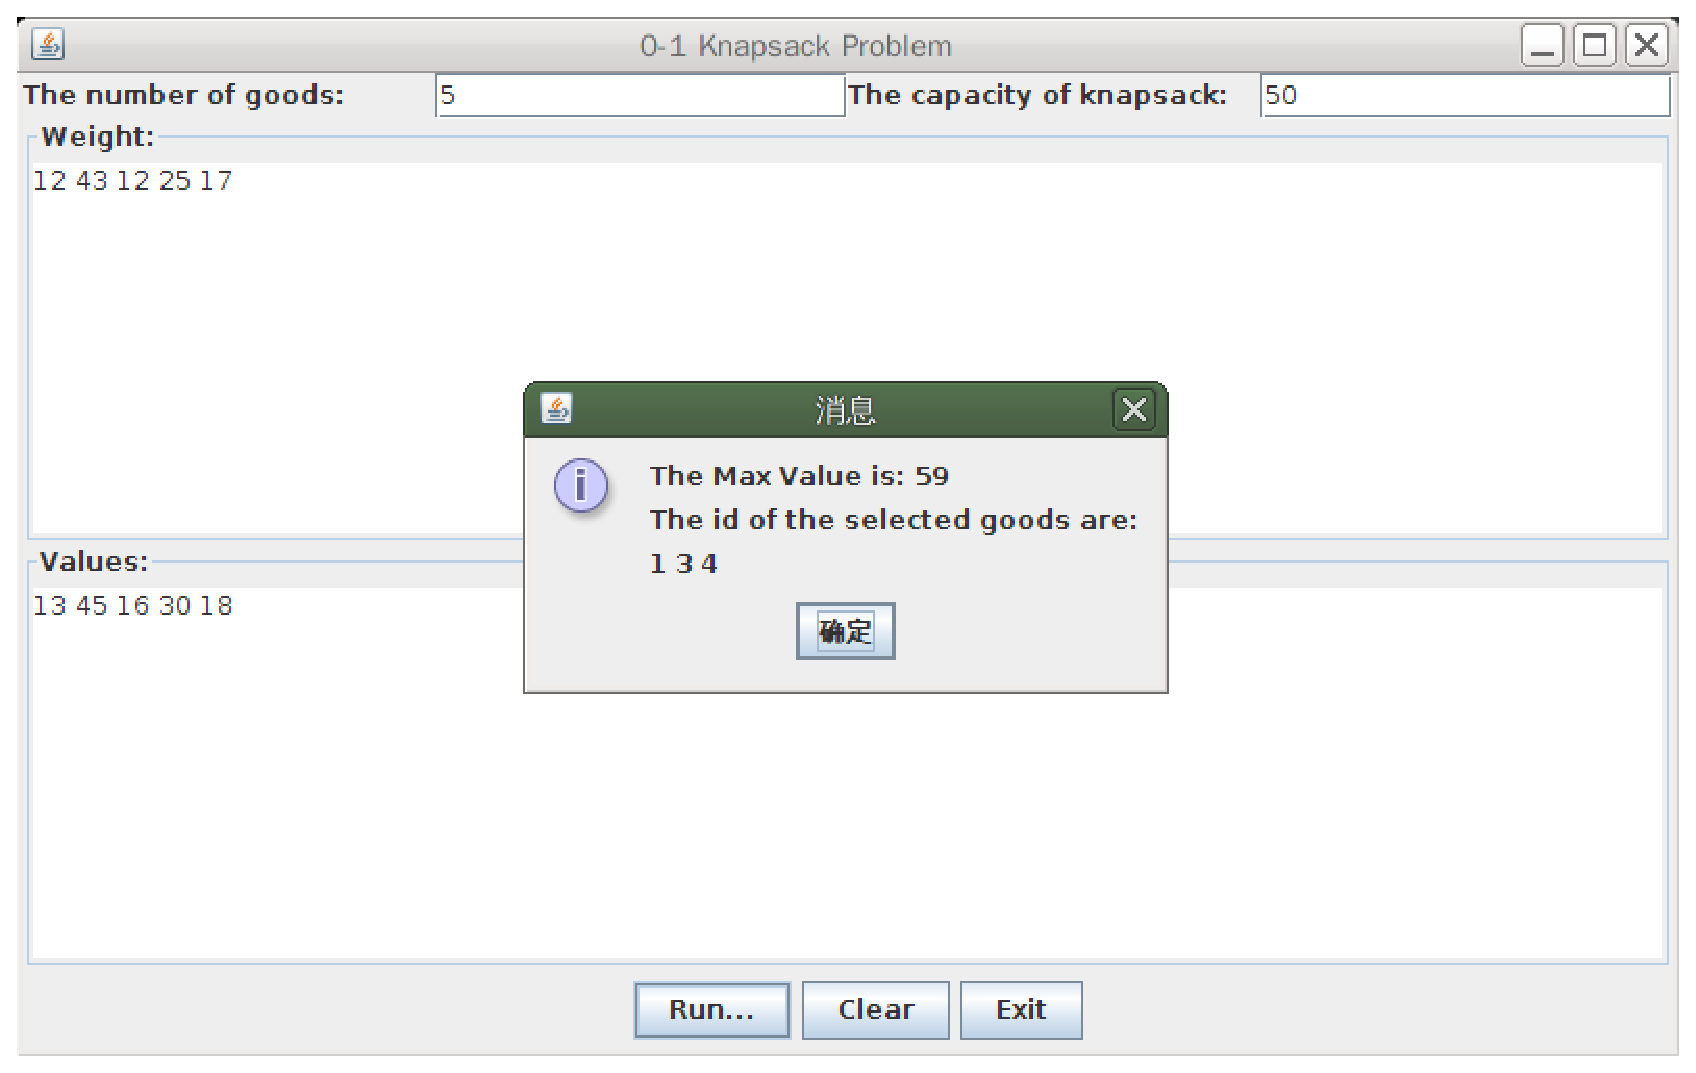
\includegraphics[height=7cm, width=12cm]{knapsack.eps}
\end{figure}

\section{Exercise 16.2-6}

可以将物品分成单位重量大小,然后按照分好的物品的价值,使用线性选择,选出前W(背包容量)大(价值大)的物品。这
就得到了最优解。但是,这种算法的时间复杂度为$O(\sum_{i=1}^{n}{w[i]})$。

分析上面的算法。对于前W大的物品,其中必然是包含若干个单位价值最大的物品的全部分块。还可能包含一个物品
的若干分块。因此,可以不对物品进行预先分成单位质量。只需要直到这个可能存在的需要分割的物品即可。

\begin{itemize}
	\item 首先,计算所有物品的价值密度(单位质量的价值)。
	\item 使用9.3节中的线性选择算法按照物品的价值密度进行选择,但事先并不确定所要选择的是
		第几大的元素。
	\item 在划分的同时,计算划分到前半部的物品的总质量。划分的时间复杂度保持不变。
	\item 按照前半部的总质量,决定下面的步骤:
	\begin{itemize}
		\item 如果前半部分的总质量大于背包容量,则继续对前半部进行查找。
		\item 如果前半部分的总质量小于背包容量,则对后半部进行查找,但背包的容量变成
			原来的容量减去前半部分的总质量。
		\item 如果前半部分的总质量等于背包容量,那么算法结束。找到最优解。
	\end{itemize}
	\item 如果算法最后停止在某一个物品上,但没有找到上面第三小步的情况。那么这个物品需要被
		分割。计算此物品前的所有物品的质量,得到所要分割的大小。进而得到最优解。
\end{itemize}

	计算所有物品的价值密度需要$\Theta(n)$的时间,中间的选择和原算法的时间复杂度一样,为
$O(n)$。最后可能出现的分割需要$\Theta(n)$。因此,算法的时间复杂度为$2\Theta(n)+O(n)=O(n)$


\section{Exercise 16.3-6}
	\begin{Lemma}\label{L1}
	$C$是一个字母集合,对于字母$c \in C$,有一个对应的频率f[c]。设$x,y,z$是$C$中三个
	频率最低的字母。那么,存在$C$的一种最优字符编码形式,使得$x,y,z$的编码长度一样且只有
	最后一位不同。
	\end{Lemma}
	\begin{Lemma}\label{L2}
	$C$是一个字母集合,对于字母$c \in C$,有一个对应的频率f[c]。设$x,y,z$是$C$中三个
	频率最低的字母。令$C'=C-\{x,y,z\}\cup\{r\}, f[r]=f[x]+f[y]+f[z]$。$T'$表示$C'$
	的一个最优前缀编码树。那么,从$T'$中用以$x,y,z$为子节点的节点代替r,得到数$T$,那么
	$T$是$C$的一棵最优前缀编码树。
	\end{Lemma}
	
	首先,可以通过类似Huffman编码的方式构造最优前缀编码树。只是,每次选择频率最小的三个节点。
构造出来的树是一棵三叉树。

	对于定理\ref{L1},可以使用课本中同样的方法证明。选择一棵最优前缀编码树$T$的最低的三个节点,
依次替换成$x,y,x$,得到的三棵树用$T',T'', T'''$表示。根据课本中的方法,可以得到:
\begin{displaymath}
\begin{array}{l}
	B(T)-B(T') \ge 0\\
	B(T')-B(T'') \ge 0\\
	B(T'')-B(T''') \ge 0\\
\end{array}
\end{displaymath} 
并且$B(T) \le B(T')$。因此,可以得到$B(T) = B(T')= B(T'')= B(T''')$。因此,最后得到的
$T'''$也是一棵最优前缀编码树。因此得证。

	对于定理\ref{L2}。同样使用课本中的证明方法。依据课本中的方法,有:
\begin{displaymath}
\begin{array}{rl}
f[x]d_{T}(x) + f[y]d_{T}(y) + f[z]d_{T}(z)& = (f[x]+f[y]+f[z])(d_{T'}(z)+1)\\
&=f[r]d_{T'}(r)+(f[x]+f[y]+f[z])\\
\end{array}
\end{displaymath}
可以得到:
\begin{displaymath}
	B(T')=B(T)-f[x]-f[y]-f[z]
\end{displaymath}

假设$T$不是$C$的最优前缀编码树,那么,存在树$T''$是$C$的最优前缀编码树,$B(T'')<B(T)$。不失
一般性,$T''$有节点$x,y,z$并且是兄弟节点。设树$T'''$是从树$T''$替换$x,y,z$为$r$得到的,
$f[r]=f[x]+f[y]+f[z]$。那么:
\begin{displaymath}
\begin{array}{rl}
B(T''')& = B(T'')-f[x]-f[y]-f[z]\\
       & < B(T)-f[x]-f[y]-f[z]\\
       & = B(T')\\
\end{array}
\end{displaymath}
这和$T'$是$C'$的最优前缀编码树矛盾。因此,T一定是C的最优前缀编码树。

\end{document}
